%%%% Proceedings format for most of ACM conferences (with the exceptions listed below) and all ICPS volumes.
\documentclass[sigconf]{acmart}
%%%% As of March 2017, [siggraph] is no longer used. Please use sigconf (above) for SIGGRAPH conferences.

%%%% Proceedings format for SIGPLAN conferences 
% \documentclass[sigplan, anonymous, review]{acmart}

%%%% Proceedings format for SIGCHI conferences
% \documentclass[sigchi, review]{acmart}

%%%% To use the SIGCHI extended abstract template, please visit
% https://www.overleaf.com/read/zzzfqvkmrfzn

\begin{document}

\title{Higher-order networks: Exploring air traffic dynamics}

% The "author" command and its associated commands are used to define the authors and their affiliations.
\author{Bradley Dice}
\email{bdice@bradleydice.com}
\orcid{0000-0002-9983-0770}
\affiliation{
  \institution{University of Michigan \\ Department of Physics}
  \city{Ann Arbor}
  \state{Michigan}
  \postcode{48109}
}

\author{Daniel McCusker}
\email{dmccuske@umich.edu}
\affiliation{
  \institution{University of Michigan \\ Applied Physics}
  \city{Ann Arbor}
  \state{Michigan}
  \postcode{48109}
}

\author{Shannon Moran}
\email{moranse@umich.edu}
\orcid{0000-0002-3579-3149}
\affiliation{
 \institution{University of Michigan \\ Department of Chemical Engineering}
  \city{Ann Arbor}
  \state{Michigan}
  \postcode{48109}
 }

\renewcommand{\shortauthors}{Dice, et al.}

% The abstract is a short summary of the work to be presented in the article.
% \begin{abstract}
% \end{abstract}

% Keywords, separate with commas.
% \keywords{higher order networks, graph mining, network dynamics, air transportation}

% \begin{teaserfigure}[b]
%   \centering
%   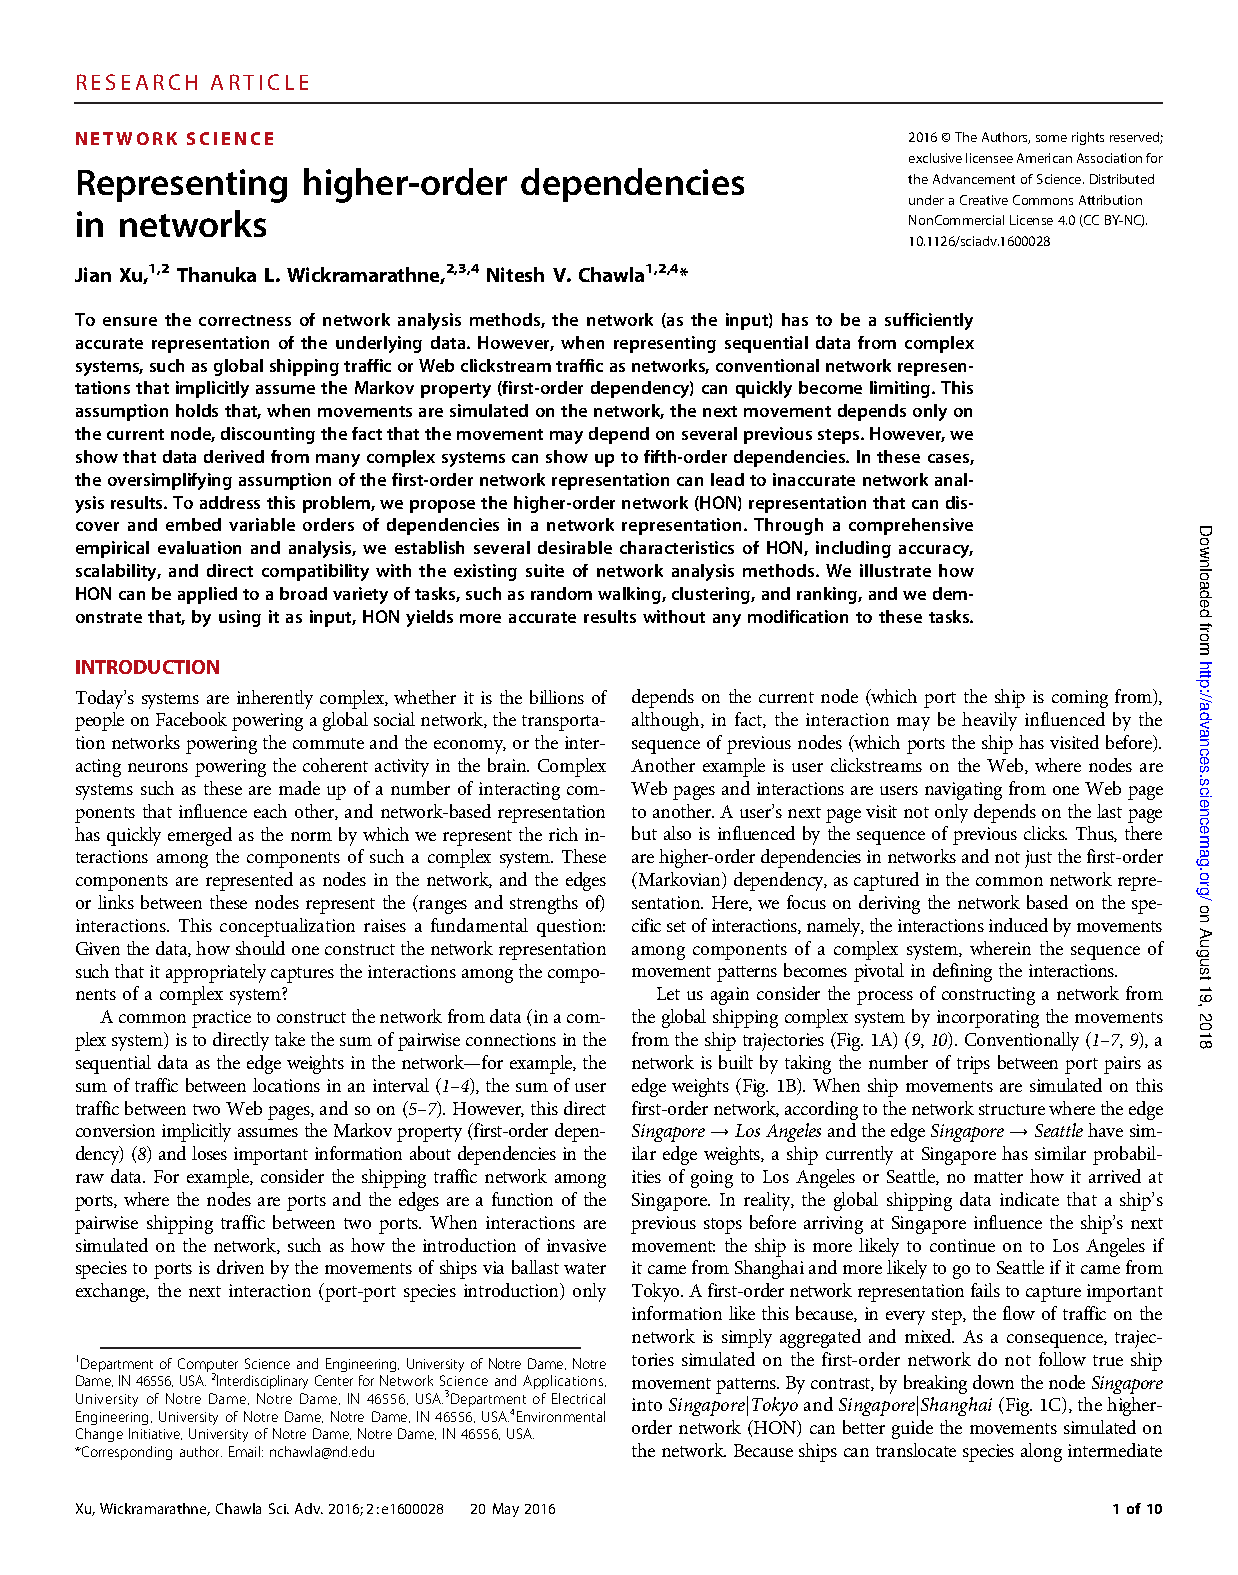
\includegraphics[width=0.7\textwidth]{HON.png}
%   \caption{Higher-order networks, visualized. source: http://www.higherordernetwork.com/}
%   \label{fig:HON}
% \end{teaserfigure}

% Show author, affiliation, and title information
\maketitle

\section{Problem definition}
Traditional network representations of data implicitly assume first-order dynamic processes. For instance, the next step of a random walker on a network depends only on its current position, and not its history. This has implications for network measures like PageRank and community detection which implement random walkers. In fact, the history of a trajectory on a network has significant bearing on predicting the trajectory's next step; for instance, a passenger flying from one city to the next is most likely to return to the first city on a round trip, rather than randomly flying to another city serviced by the second airport. Implementing higher-order network representations that account for such histories is key to achieving an accurate graph-level understanding of network data. 

We propose applying the \texttt{BuildHON+} algorithm of Xu \textit{et al.} in order to build a \textbf{higher-order network representation of airline itinerary data} \cite{Xu2017, AirlineData}. We will study the resulting \textbf{community structure using the MapEquation framework}, and compare the results to a first-order and a fixed second-order Markov network to illustrate the implications of higher-order representations. 

\section{Challenges}
First, why do we need higher-order networks, or HONs?
HONs break up the physical nodes of the network into \textit{state nodes} which incorporate trajectory history.
For instance, the node \textit{Atlanta} may be broken up into \textit{Atlanta | Chicago}, \textit{Atlanta | New York}, etc. for a fixed second-order representation.

However, a challenge in such fixed-order representation is the combinatorial explosion as the order $k$ increases. Moreover, such networks suffer from overfitting when not all state nodes are statistically significant. For these reasons, we've chosen to adopt the HON representation method of Xu \textit{et al.}, a variable-order method which determines only the statistically significant state nodes. 

\section{Related prior work}
% discuss the shortcomings of these papers
We have identified three core parts of this project, building upon prior literature: (1) use of the airline data set as a test case for higher-order network (HON) methods, (2) representing data sets as HONs, and (3) identifying communities in HONs.


\subsection{Prior airline analysis}

Past work on the DB1B airline itinerary data set has used a fixed second-order network on data from 2011 Q1 to Q3 \cite{Rosvall2014}. This data set was a benchmark for their HON model which shows much less entropy in the MapEquation model for a second-order network compared to a first-order network.

This study found that 79\% of the paths in the data were of length 3 or greater, though the network used for analysis was strictly second order. We hope to expand on this by comparing different, longer subsets of the entire data set of 100 quarters (instead of just 3 quarters) to extract longer-ranged changes in communities that may be attributable to market shifts, mergers and acquisitions, and global events affecting the airline industry such as terrorism. This approach is subject to change, pending computational difficulty of working with such data sets.

\subsection{Methods for forming higher-order networks from trajectory data}

There are two primary ways to form higher-order networks from trajectory-like data. The simplest approach is to take a fixed order $k$ and divide each of the graph's $N$ physical nodes into ``state nodes'' representing trajectories of length $k$ ending with that physical node. These state nodes encode the history of a trajectory, e.g. $\vec{hij}$ might represent a state node for the physical node $j$ which had previously visited $h$ and $i$ before arriving at $j$ \cite{Rosvall2014}. Fixed order representations must ignore trajectories with total length less than $k$, since the trajectory cannot be represented in a second order state node \cite{Rosvall2014}. Additionally, the number of state nodes must increase as $N^k$ to record all possible trajectories, limiting this approach to small $k$ (typically 2) \cite{Rosvall2014}. A more complex representation is that of Xu \textit{et al.} \cite{Xu2016}, later improved to be parameter-free \cite{Xu2017}, where the order is determined dynamically from data: state nodes represent trajectories of variable length, and higher-order state nodes are created if and only if their creation is statistically significant for the network's predictive power. This method allows for a sparse representation that can capture higher-order dynamics than fixed-order models, which are computationally constrained by the explosive growth in state nodes as $k$ increases. As the authors clarify, ``if the dependency is assumed as fixed second order, it could be redundant when first-order dependencies are sufficient and could be insufficient when higher-order dependencies exist'' \cite{Xu2016}.

\subsection{Clustering or other centrality algorithms for higher-order networks} 

An insight of Xu \textit{et al.} is that typical network analysis methods, such as clustering, centrality, and ranking, can be applied to study higher-order networks, once a network of higher-order state nodes has been produced \cite{Xu2016}. For instance, they apply MapEquation, a clustering algorithm based on the entropy of random walks, to a shipping data set. By merging the state nodes into physical nodes at the end, they naturally reveal a rich overlapping community structure, with important implications for studying the transmission of invasive species. This structure is hidden in the first-order network analysis.

\section{Choice of data set}
We were interested in choosing a data set representing time-based trajectories. Additionally, we wanted to choose one data set and apply multiple methods.

We considered data sets referenced in \cite{Scholtes2017} and the network database maintained by Prof. Clauset at UC Boulder \cite{Clauset2016}. We chose data from the Airline Origin and Destination Survey (DB1B) collected by the Office of Airline Information of the Bureau of Transportation Statistics, because of its richness, long time span, and use in other papers in the field \cite{AirlineData}. The data include origin, destination, and other itinerary details of passengers transported. This database can be used to describe air traffic patterns, air carrier market shares, and passenger flows.

We have already downloaded the complete data set, including \textit{Coupon}, \textit{Market}, and \textit{Ticket} data aggregated on a quarterly basis from 1993 Q1 to 2018 Q3. The data size is 25 GB in zipped files. This includes 837 million observations of itinerary coupons, 507 million observations of origin/destination markets, and 286 million observations of airline tickets. We have some experience using PySpark\footnote{https://spark.apache.org/docs/latest/api/python/index.html}, and plan to use this framework for our data analysis because of its compatibility with our university's Hadoop cluster, scalability, and ease of use for rapid prototyping in Python.

\section{Proposed approach}

\subsection{Converting data sets into HONs}
We plan to use the improved \texttt{BuildHON+} algorithm of Xu \textit{et al.} \cite{Xu2017} to build a higher-order network of this data. We will subset the data to explore the network effects of real-world events such as major airline mergers (e.g. American Airlines and TWA, 2001; Delta and Northwest Airlines, 2008-2010; American Airlines and US Airways, 2013-2015). First, events will be merged on their unique identifiers to form trajectories. These trajectories are the input for the \texttt{BuildHON+} algorithm. Previous work on DB1B data by Rosvall \textit{et al.} made some helpful assumptions about paths' endpoints (e.g. choice of memory nodes) that we plan to replicate in our analysis for simplicity and reproducibility \cite{Rosvall2014}.

\subsection{Implementing HON representation using Python}
There is an open-source Python implementation\footnote{https://github.com/xyjprc/hon} of the HON algorithm of Xu \textit{et al.} but our preliminary reviews of that code suggest that we may need to re-implement a portion of it for improved performance and scalability via PySpark's \texttt{DataFrame}s and resilient distributed data sets (RDDs) \cite{Xu2016,Xu2017}. The algorithm is not too complex, so this should be within a reasonable scope for this project. We plan to vary the maximum HON order $k$ from 1 to 5. The algorithm's time complexity is not strongly dependent on $k$ after a certain point, as seen in Table 1 of the HON paper where the run time of $k = 3$ and $k = 5$ differ by only 8\% \cite{Xu2016}. This is because there are typically far fewer correlations of high order than low order, so testing correlations of order $k$ for extension to order $k+1$ gets cheaper as the number of correlations decreases.

\subsection{Methods used for cluster analysis of flight data HON.} We plan to implement MapEquation, the random walker-based community detection algorithm, to detect overlapping communities in the airport nodes \cite{Rosvall2009}. This will allow us to directly compare our results to the fixed second-order airline representation in Rosvall's 2014 paper, as well as to the overlapping communities in shipping data in Xu's original HON paper \cite{Rosvall2014, Xu2016}. Xu's second paper \cite{Xu2017}, which introduces the \texttt{BuildHON+} algorithm, also uses anomaly detection. We might also investigate the airline network dynamics using this technique, and use the results, in addition to those from MapEquation, to build a comprehensive, qualitative description of the dynamics on the airline network.

\begin{figure}
    \centering
    % \includegraphics[width=0.5\textwidth]{clustering.png}
    % \captions{Results of port community detection with MapEquation on shipping data for \textbf{(A)} a first-order network and \textbf{(B)} a HON.}
    \includegraphics[width=0.5\textwidth]{air_modules.jpg}
    \caption{An example of community detection using the MapEquation framework on airline traffic \cite{Rosvall2014}. While Las Vegas and Atlanta are their own communities in first-order Markov dynamics (a), using second-order Markov dynamics (b) we see communities (color) of "round-trip" tickets (line weight) to Las Vegas represented (and Las Vegas is included in 8 communities). Further discussion in text.}
    \label{fig:clustering}
\end{figure}

\section{Evaluation of methods}
% SHANNON What output do we expect from the cluster analysis? Consider adding in a representative image from one of the papers we cite. 
% Some nice videos/graphics here http://www.higherordernetwork.com/
% Reproduce the fixed second-order result of Rosvall et al. and show the improvements from HON?

We will evaluate our results by benchmarking them to those found in the literature. At minimum our goal will be to replicate previous findings on flight data \cite{Rosvall2014} and find communities that are not detectable without higher-order network topology.

As an example of what we will be comparing our work against, we present a case study from the literature in Figure \ref{fig:clustering}\cite{Rosvall2014}.
For a subset of air traffic data between US cities, a first-order Markov model assigns Las Vegas and Atlanta to their own singular communities (Figure \ref{fig:clustering}a).
However, a second-order Markov model captures the ``two-step return rate'' that allows communities to be built based on short round-trip trajectories.
Of interesting note in Figure \ref{fig:clustering}b, Las Vegas is part of 8 communities while Atlanta is part of only 2.
This is likely explained by Atlanta being a transfer hub while Las Vegas is a tourist destination, something only captured by a second order network. While some communities appear to be regionally close, others don't make sense (e.g. \textit{Las Vegas | NYC} being in the same community as Atlanta).
We suspect this would be improved with a variable $k$ approach, and aim to test this hypothesis in our project.

% Example on freight shipping data: ``Ports tightly coupled by frequent shipping in a cluster are likely to introduce non-native species to each other. MapEquation (38) is used for clustering, and different colors represent different clusters. (A) Clustering on the first-order network. Although Valletta and Malta Freeport are local and international ports, respectively, the clustering result does not distinguish the two. (B) Clustering on HON. The overlapping clusters indicate how international ports (such as Malta Freeport) may suffer from species invasions from multiple sources.'' \cite{Xu2016}

%\section{Distribution of work}
%Each group member (Bradley, Dan, and Shannon) contributed equally to the proposal. All group members agreed unanimously on the topic. Among the group members, slight biases in work distribution were: Bradley in the data set identification, Dan in the literature review, and Shannon in the writing of the proposal and presentation. However, all team members contributed to all parts of the report. %Moving forward, we will have more defined modules on the project.

\newpage
\bibliographystyle{ACM-Reference-Format}
\bibliography{proposal}

\appendix
% Any appendix sections would go here

\end{document}
